\section{Mechanical Model of a Quantum Field}

To build intuition for quantum fields, it is useful to begin with a simple mechanical system: a chain of coupled elastic strings. This model arises as the \textit{continuum limit} of a one-dimensional lattice of \(N\) atoms, and already captures many of the essential features of field theories.  

We consider a \textbf{meta-stable} system, meaning that its configuration does not change drastically under the action of a small perturbing force.\footnote{In fact, every physical system is meta-stable in this sense: if a small perturbation could radically alter its configuration, it could not persist in a stable state.} Thus, there must exist a restoring force that drives the system back toward equilibrium.  

For a small displacement \(y\) from equilibrium, the restoring force can be expanded in a Taylor series:
\[
  F(y) = F(0) + \left.\frac{dF}{dy}\right|_{y=0} y + \dots 
       = -|\kappa|\, y + \mathcal{O}(y^2),
\]
where we set \(F(0) = 0\) (no force at equilibrium) and require \(\left.\tfrac{dF}{dy}\right|_{y=0} = -|\kappa| < 0\) (restoring behavior). The linear term dominates for sufficiently small displacements, showing that any meta-stable system can be modeled, to first approximation, as a collection of coupled harmonic oscillators.  

The simplest realization is a chain of \(N\) identical atoms, each of mass \(m\), connected by springs with spring constant \(\kappa\) and arranged along a line with equilibrium spacing \(\Delta\). The total length of the chain is
\[
  L = N \Delta.
\]
The displacement of the \(i\)-th atom from its equilibrium position will be denoted by \(y_i(t)\). For simplicity, we restrict ourselves to transverse displacements along the \(y\)-axis, keeping the equilibrium positions along the \(x\)-axis fixed.

\begin{figure}[H]
\begin{minipage}{0.45\textwidth}
\centering
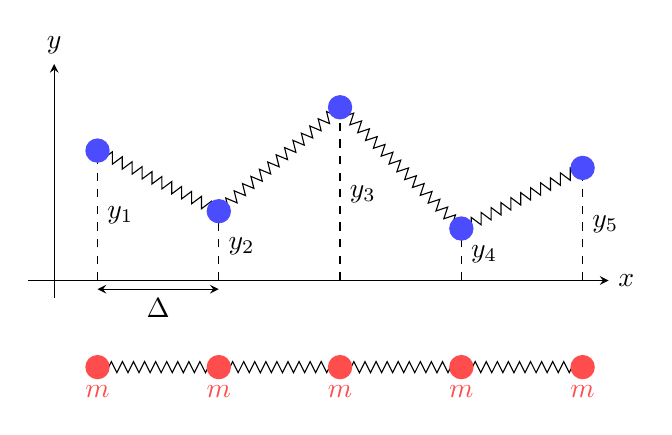
\begin{tikzpicture}[scale=1.1,>=stealth]

  % Horizontal spacing between masses
  \def\Deltax{1.4}

  % Random vertical positions (displacements)
  \def\yA{0.5}
  \def\yB{-0.2}
  \def\yC{1.0}
  \def\yD{-0.4}
  \def\yE{0.3}

  % Reference axes
  \draw[->] (-0.5,-1.2) -- (-0.5,1.5) node[anchor=south]{$y$};
  \draw[->] (-0.8,-1.0) -- (5*\Deltax-1.1,-1.0) node[anchor=west]{$x$};

  % --- Upper part: masses at different y ---
  % Mass vertical positions
  \coordinate (m1) at (0,\yA);
  \coordinate (m2) at (\Deltax,\yB);
  \coordinate (m3) at (2*\Deltax,\yC);
  \coordinate (m4) at (3*\Deltax,\yD);
  \coordinate (m5) at (4*\Deltax,\yE);

  % Springs (zigzag lines)
  \draw[decorate,decoration={zigzag,segment length=4pt,amplitude=2pt}] (m1) -- (m2);
  \draw[decorate,decoration={zigzag,segment length=4pt,amplitude=2pt}] (m2) -- (m3);
  \draw[decorate,decoration={zigzag,segment length=4pt,amplitude=2pt}] (m3) -- (m4);
  \draw[decorate,decoration={zigzag,segment length=4pt,amplitude=2pt}] (m4) -- (m5);

  % Segments and spacings
  \foreach \i/\y in {1/\yA, 2/\yB, 3/\yC, 4/\yD, 5/\yE} {
    \draw[dashed] (\i*\Deltax-\Deltax,-1) -- (\i*\Deltax-\Deltax,\y) node[midway,right] {$y_{\i}$};
  }
  \draw[<->] (0,-1.1) -- (\Deltax,-1.1) node[midway,below] {$\Delta$};

  % Masses (blue circles)
  \foreach \m in {m1,m2,m3,m4,m5}{
    \fill[blue!70] (\m) circle (4pt);
  }

  % --- Lower part: horizontal chain ---
  \begin{scope}[yshift=-2cm]
    % Horizontal positions
    \coordinate (n1) at (0,0);
    \coordinate (n2) at (\Deltax,0);
    \coordinate (n3) at (2*\Deltax,0);
    \coordinate (n4) at (3*\Deltax,0);
    \coordinate (n5) at (4*\Deltax,0);

    % Springs
    \draw[decorate,decoration={zigzag,segment length=4pt,amplitude=2pt}] (n1) -- (n2);
    \draw[decorate,decoration={zigzag,segment length=4pt,amplitude=2pt}] (n2) -- (n3);
    \draw[decorate,decoration={zigzag,segment length=4pt,amplitude=2pt}] (n3) -- (n4);
    \draw[decorate,decoration={zigzag,segment length=4pt,amplitude=2pt}] (n4) -- (n5);

    % Masses (red circles)
    \foreach \n in {n1,n2,n3,n4,n5}{
      \fill[red!70] (\n) circle (4pt);
      \node[red!70,below=3pt] at (\n) {$m$};
    }
  \end{scope}

\end{tikzpicture}
\end{minipage}
\hfill
\begin{minipage}{0.45\textwidth}
\(y_i=0\) is the equilibrium position of the \(i\)-th atom. The springs exert restoring forces proportional to the relative displacements of neighboring atoms: each atom is under the influence of the neighboring springs, describing a local interaction.

\(y_i\neq0\) describes the small oscillations around the equilibrium position: transverse \textbf{excitations} of the lattice.
\end{minipage}
\end{figure}

In the limit \(N\to\infty\) and \(\Delta \to 0\) with \(L\) fixed, the discrete index \(i\) becomes a continuous spatial coordinate and the displacements \(y_i(t)\) become a continuous field \(\phi(x,t)\). This \textbf{continuum limit} transforms the system of coupled oscillators into a continuous field, allowing us to understand the dynamics of fields in terms of familiar mechanical concepts.

\subsection*{Dynamical Analysis}

To study the dynamics of the chain we employ the Euler--Lagrange equations.  
The Lagrangian of the system is constructed as the difference between the kinetic and potential energy contributions of each atom:
\[
  L = \sum_{j=1}^N \left[ \frac{1}{2} m \dot{y}_j^2 - \frac{1}{2} \kappa \left(\frac{y_j - y_{j+1}}{\Delta}\right)^2 \right],
\]
where we impose periodic boundary conditions \(j \to j+N\).\footnote{In other words, the first and the last atoms in the chain interact with each other.}  

We are assuming small oscillations around the equilibrium configuration, such that the relative displacement between neighboring atoms is small compared to the natural lattice spacing \(\Delta\):
\[
  \frac{y_j - y_{j+1}}{\Delta} \ll 1.
\]

It is worth noting that the coupling constant \(\kappa\) has the dimension of an energy, and can be written as
\[
  \kappa = m v^2,
\]
where \(v\) is a characteristic velocity associated with the propagation of disturbances along the chain. With this identification, the Lagrangian becomes
\[
  L = \frac{1}{2}m \sum_{j=1}^{N} \left[ \dot{y}_j^2(t) 
  - v^2\left(\frac{y_j - y_{j+1}}{\Delta}\right)^2  \right],
\]
where the first term corresponds to the kinetic energy of the atoms, while the second encodes the elastic potential energy due to the coupling between neighbors.  

The time evolution of the system is obtained by applying the principle of least action: 
the motion is such that the variation of the action vanishes,
\[
  S = \int L \, \mathrm{d}t, \qquad \delta S = 0,
\]
which leads to the Euler--Lagrange equations governing the dynamics of the chain. 
Recalling the general form
\[
  \frac{\mathrm{d}}{\mathrm{d} t} \frac{\partial L}{\partial \dot{y}_j} 
  = \frac{\partial L}{\partial {y}_j}, 
  \qquad j = 1, \dots , N,
\]
we obtain the governing equations of motion:
\[
  \ddot{y}_j (t) 
  = -\,v^2 \left(\frac{2y_j - y_{j+1} - y_{j-1}}{\Delta^2}\right).
\]
This result clearly describes a system of coupled harmonic oscillators: the displacement of the \(j\)-th atom is influenced not only by its own position but also by the relative positions of its nearest neighbors, \((j+1)\) and \((j-1)\). 
In other words, each atom is bound to oscillate around equilibrium under the restoring force arising from the springs that connect it to its neighbors.

Solving such a system directly is not convenient, since the equations are not independent. However, there is a natural way to simplify the problem by exploiting the translational symmetry of the lattice. The key idea is to perform a \textit{discrete Fourier transform} of the displacements, which allows us to rewrite the dynamics in terms of normal modes of oscillation. Since \(y_j(t)\) has to be periodic (\(y_j(t) = y_{j+N}(t)\)), we can write:
\[
  y_j(t) = \frac{1}{\sqrt{N}} \sum_{\sigma=1}^{N} e^{i\frac{2\pi}{N}\sigma j} \tilde{y}_{\sigma}(t).
\] 
In this new representation, each mode corresponds to a collective oscillation of the entire chain with a definite wavelength. From a mathematical perspective, this amounts to diagonalizing the interaction matrix: the coupling between neighbors is replaced by a set of independent equations for the Fourier modes. In physical terms, the Fourier transform identifies the proper "coordinates" in which the energy of the system can be expressed as a sum of independent contributions, one for each mode.\footnote{In other words, instead of tracking the motion of individual atoms, which are strongly coupled, we describe the system in terms of delocalized excitations (the normal modes), each evolving independently. This step paves the way to the field interpretation: in the continuum limit, these modes will be interpreted as excitations of a quantum field.}

Now, by substituting in the equation of motion, we can decouple the system:
\[
\begin{aligned}
  \frac{1}{\sqrt{N}} \sum_{\sigma=1}^{N} e^{i\frac{2\pi}{N}\sigma j} \ddot{\tilde{y}}_{\sigma} &= \frac{-1}{\sqrt{N}} \left(\frac{v}{\Delta}\right)^2 \left[ 2 \sum_{\sigma=1}^{N} e^{i\frac{2\pi}{N}\sigma j} \tilde{y}_{\sigma} - \sum_{\sigma=1}^{N} e^{i\frac{2\pi}{N}\sigma (j-1)} \tilde{y}_{\sigma} - \sum_{\sigma=1}^{N} e^{i\frac{2\pi}{N}\sigma (j+1)} \tilde{y}_{\sigma}\right]\\
  &= \frac{-1}{\sqrt{N}} \left(\frac{v}{\Delta}\right)^2 \sum_{\sigma=1}^{N} e^{i\frac{2\pi}{N}\sigma j} \tilde{y}_{\sigma} \left[ 2 - e^{-i\frac{2\pi}{N}\sigma} - e^{i\frac{2\pi}{N}\sigma}\right]\\
  &= \frac{-1}{\sqrt{N}} \left(\frac{v}{\Delta}\right)^2 \sum_{\sigma=1}^{N} e^{i\frac{2\pi}{N}\sigma j} \tilde{y}_{\sigma} \left[ 2 - 2 \cos(\frac{2\pi}{N}\sigma)\right]\\
  \iff \ddot{\tilde{y}}_{\sigma}(t) &= - 2 \frac{v^2}{\Delta^2} \left[ 1 - \cos(\frac{2\pi}{N}\sigma)\right] \tilde{y}_{\sigma}(t) = - \left( \frac{2v}{\Delta} \sin(\frac{\pi\sigma}{N}) \right)^2 \tilde{y}_{\sigma}(t),
\end{aligned}
\]
where we have made use of the trigonometric identity 
\((1 - \cos(2\theta)) = 2\sin^2(\theta)\). This leads to the following set of equations for the Fourier modes:
\[
\begin{aligned}
  \ddot{\tilde{y}}_{\sigma}(t) &= - \omega^2_{\sigma}\, \tilde{y}_{\sigma}(t),
  \quad && \forall \, \sigma = 1,2,\dots,N, \\
  \omega_{\sigma} &= \frac{2v}{\Delta} \, \sin\!\left(\frac{\pi\sigma}{N}\right).
\end{aligned}
\]
%
Each Fourier component \(\tilde{y}_{\sigma}(t)\) evolves independently and satisfies the equation of a simple harmonic oscillator with characteristic frequency \(\omega_{\sigma}\). 
In other words, the original coupled system of atoms has been diagonalized into a set of \(N\) decoupled oscillators, each associated with a normal mode of vibration. 

The general solution for each mode is therefore given by a linear combination of oscillatory functions:
\[
  \tilde{y}_{\sigma}(t) 
  = A_{\sigma} e^{-i \omega_{\sigma} t} + B_{\sigma} e^{+i \omega_{\sigma} t},
\]
where the constants \(A_{\sigma}\) and \(B_{\sigma}\) are determined by the initial conditions. 
Physically, these modes correspond to standing waves propagating through the chain, each characterized by a discrete wave number and its corresponding frequency.

In practice, we will keep only the negative exponential,
\[
  \tilde{y}_{\sigma}(t) = A_{\sigma} e^{-i \omega_{\sigma} t},
\]
since the positive-frequency solution is automatically recovered as the complex conjugate. 
This choice avoids redundancy and is particularly convenient when later quantizing the system, because creation and annihilation operators will naturally emerge from the decomposition into \(e^{-i\omega t}\) and its conjugate.

Now we can plug the solution for the Fourier modes back into the inverse transform in order to recover the displacement of the \(j\)-th atom:
\[
\begin{aligned}
    y_j(t) &= \frac{1}{\sqrt{N}} \sum_{\sigma=1}^{N} e^{i\frac{2\pi}{N}\sigma j} \tilde{y}_{\sigma}(t) \\
    &= \frac{1}{\sqrt{N}} \sum_{\sigma=1}^{N} A_{\sigma} e^{i \left( \frac{2\pi}{N}\sigma j - \omega_{\sigma} t \right)} \\
    &= \frac{1}{\sqrt{N}} \sum_{\sigma=1}^{N} A_{\sigma} e^{i \left( \frac{2\pi}{N}\frac{\sigma}{\Delta} (\Delta j) - \omega_{\sigma} t \right)},
\end{aligned}
\]
Here we have reintroduced the lattice spacing \(\Delta\), so that the quantity \(\Delta j\) corresponds exactly to the physical position \(x\) of the \(j\)-th atom along the chain. 

This expression shows that the displacement of each atom can be written as a linear superposition of plane waves (like \textit{sound waves}). In particular, the system supports \(N\) different wave numbers, each corresponding to one Fourier mode:
\[
    \kappa_{\sigma} = \frac{2\pi}{N} \frac{\sigma}{\Delta} = \frac{2\pi}{\lambda_{\sigma}}, \qquad \sigma = 1,2,\dots,N,
\]
with associated discrete wavelengths
\[
    \lambda_{\sigma} = \frac{N\Delta}{\sigma} = N\Delta, \, \frac{N\Delta}{2}, \dots, \Delta.
\]

\begin{remark}
    The propagation speed of each mode is obtained as the ratio between its frequency and its wave number:
    \[
        v_{\sigma} = \frac{\omega_{\sigma}}{\kappa_{\sigma}}
        = \frac{\tfrac{2v}{\Delta}\,\sin\!\left(\tfrac{\pi\sigma}{N}\right)}{\tfrac{2\pi}{N}\tfrac{\sigma}{\Delta}}
        = v \,\frac{N}{\pi\sigma} \,\sin\!\left(\tfrac{\pi\sigma}{N}\right).
    \]
    Introducing the parameter \(\theta_{\sigma} = \tfrac{\pi\sigma}{N}\), this can be written in the compact form
    \[
        v_{\sigma} = v\,\frac{\sin(\theta_{\sigma})}{\theta_{\sigma}}.
    \]
    This result shows that each Fourier mode propagates with a distinct phase velocity, depending on the ratio \(\sigma/N\). 
    In the continuum limit \(N \to \infty\) with \(\sigma/N \to 0\), one has \(\theta_{\sigma} \to 0\) and therefore 
    \[
        \lim_{\theta_{\sigma}\to 0} \frac{\sin(\theta_{\sigma})}{\theta_{\sigma}} = 1,
    \]
    so all modes propagate with the same velocity \(v_{\sigma} \sim v\). This recovers the expected propagation speed of sound waves in the continuous chain.
\end{remark}

\begin{remark}
    The actual number of independent vibrational degrees of freedom is \(N-1\), since the \(N\)-th mode corresponds to a zero frequency:
    \[
        \omega_{\sigma=N} = \frac{2v}{\Delta}\,\sin\!\left(\pi \frac{N}{N}\right) = 0.
    \]
    This means that \(\tilde{y}_N(t)\) does not oscillate in time. Physically, this mode represents a uniform translation of the entire chain, where all atoms are displaced by the same amount. As such, it does not contribute to the internal vibrational dynamics, and the only genuine oscillatory modes are the first \(N-1\).
\end{remark}

\begin{figure}[H]
\begin{minipage}{0.5\textwidth}
Moreover we can show that the waves with \(\sigma = s\) and \(\sigma = N-s\) in general have the same frequency \(\omega_s\), since:
\[
\begin{aligned}
    \omega_{N-s} &= \frac{2v}{\Delta}\,\sin\!\left(\pi \frac{N-s}{N}\right)\\
    &= \frac{2v}{\Delta}\,\sin\!\left(\pi -\frac{\pi s}{N}\right)\\ 
    &= \frac{2v}{\Delta}\,\sin\!\left(\frac{\pi s}{N}\right) = \omega_s.
\end{aligned}
\]
\end{minipage}
\hfill
\begin{minipage}{0.45\textwidth}
\centering
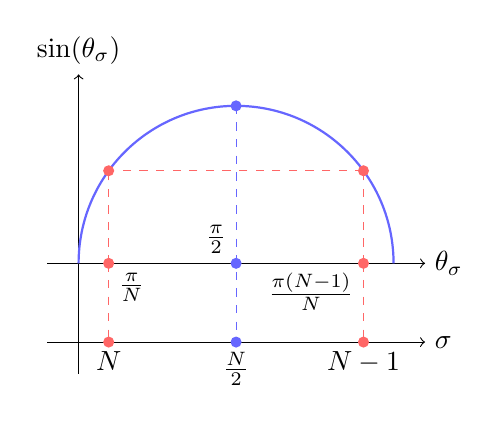
\begin{tikzpicture}[scale=2]
    \draw[->] (-0.2,0) -- (2.2,0) node[right] {$\theta_{\sigma}$};
    \draw[->] (-0.2,-0.5) -- (2.2,-0.5) node[right] {$\sigma$};
    \draw[->] (0,-0.7) -- (0,1.2) node[above] {$\sin(\theta_{\sigma})$};

    \draw[thick, blue!60] (0,0) arc[start angle=180,end angle=0,radius=1];

    \def\N{5}
    \def\xone{pi/\N}
    \def\xtwo{pi*(\N-1)/\N}

    \coordinate (A) at ({1+cos(180*\xone/pi)},{sin(180*\xone/pi)});
    \coordinate (B) at ({1+cos(180*\xtwo/pi)},{sin(180*\xtwo/pi)});
    \coordinate (-A) at ({1+cos(180*\xone/pi)},-0.5);
    \coordinate (-B) at ({1+cos(180*\xtwo/pi)},-0.5);

    \draw[dashed, red!60] (A|-0,0) -- (A);
    \draw[dashed, red!60] (B|-0,0) -- (B);
    \draw[dashed, red!60] (A|-0,0) -- (-A);
    \draw[dashed, red!60] (B|-0,0) -- (-B);
    \draw[dashed, red!60] (A) -- (B);
    \draw[dashed, blue!60] (1,1) -- (1,-0.5);

    \node[below left] at (A|-0,0) {$\frac{\pi(N-1)}{N}$};
    \node[below right] at (B|-0,0) {$\frac{\pi}{N}$};    
    \node[below] at (A|-0,-0.5) {$N-1$};
    \node[below] at (B|-0,-0.5) {$N$};
    \node[above left] at (1,0) {$\frac{\pi}{2}$};
    \node[below] at (1,-0.5) {$\frac{N}{2}$};

    \fill[red!60] (A) circle (1pt);
    \fill[red!60] (B) circle (1pt);
    \fill[red!60] (A|-0,0) circle (1pt);
    \fill[red!60] (B|-0,0) circle (1pt);
    \fill[red!60] (A|-0,-0.5) circle (1pt);
    \fill[red!60] (B|-0,-0.5) circle (1pt);
    \fill[blue!60] (1,0) circle (1pt);
    \fill[blue!60] (1,1) circle (1pt);
    \fill[blue!60] (1,-0.5) circle (1pt);
\end{tikzpicture}
\end{minipage}
\end{figure}

We can interpret the two modes with the same frequency as forming a single complex degree of freedom. This interpretation is supported by the observation that the original variable \(y_j\) is real, even though it is expressed as a sum of complex exponentials:
\[
  \begin{aligned}
    y_j(t) &= \frac{1}{\sqrt{N}} \sum_{\sigma=1}^{N} e^{i\frac{2\pi}{N}\sigma j} \tilde{y}_{\sigma}(t), \\
    y_j^*(t) &= \frac{1}{\sqrt{N}} \sum_{\sigma=1}^{N} e^{-i\frac{2\pi}{N}\sigma j} \tilde{y}_{\sigma}^*(t). \\
  \end{aligned}
\]
Thus, by requiring that the two expressions coincide, we can compute:
\[
\begin{aligned}
    \sum_{\sigma=1}^{N} e^{i\frac{2\pi}{N}\sigma j} \tilde{y}_{\sigma}(t) &= \sum_{\sigma=1}^{N} e^{-i\frac{2\pi}{N}\sigma j} \tilde{y}_{\sigma}^*(t),\\
    \sum_{\sigma=N-1}^{0} e^{i\frac{2\pi}{N}(N-\sigma) j} \tilde{y}_{N-\sigma}(t) &= \sum_{\sigma=1}^{N} e^{-i\frac{2\pi}{N}\sigma j} \tilde{y}_{\sigma}^*(t),\\
    \sum_{\sigma=N-1}^{0} e^{i2\pi j} e^{-i\frac{2\pi}{N}\sigma j} \tilde{y}_{N-\sigma}(t) &= \sum_{\sigma=1}^{N} e^{-i\frac{2\pi}{N}\sigma j} \tilde{y}_{\sigma}^*(t),\\
    \sum_{\sigma=N-1}^{0} \tilde{y}_{N-\sigma}(t) &= \sum_{\sigma=1}^{N} \tilde{y}_{\sigma}^*(t),\\
    \sum_{\sigma=1}^{N} \tilde{y}_{N-\sigma}(t) &= \sum_{\sigma=1}^{N} \tilde{y}_{\sigma}^*(t),
\end{aligned}
\]
which lead us to conclude that \(\tilde{y}_{N-\sigma}(t) = \tilde{y}_{\sigma}^*(t)\).

Now we are in a position to compute the total number of independent vibrational degrees of freedom. To do so, we must distinguish two cases:  
\begin{itemize}  
  \item \textbf{If \(N\) is even (\(N = 2l\))}, the total number of pairs of harmonic oscillators with the same frequency (denoted by \(m\)) is  
  \[
    m = \frac{2l - 2}{2} = l - 1 .
  \]  
  In this case we have to exclude the modes \(\sigma = N\) and \(\sigma = \tfrac{N}{2}\). The reason is that, when \(N\) is even, the mode with index \(\sigma = \tfrac{N}{2}\) is self-conjugate, since it coincides with its complementary mode \(\sigma = N - \tfrac{N}{2} = \tfrac{N}{2}\).  

  \item \textbf{If \(N\) is odd (\(N = 2l+1\))}, the total number of such oscillator pairs is  
  \[
    m = \frac{(2l+1) - 1}{2} = l .
  \]  
  Here the only index that must be removed is \(\sigma = N\), since \(\tfrac{N}{2}\) is not an integer and therefore does not correspond to any mode index.  
\end{itemize}  
The two oscillators associated with the same frequency can be regarded as components of a single complex degree of freedom. In this representation, the physical displacement corresponds to the real part of the complex variable, while the imaginary part encodes the redundant conjugate mode.

We could now exploit the solutions obtained in the new basis to diagonalize the Hamiltonian, since the transformation allows us to rewrite the Hamiltonian in terms of independent normal modes, each of which behaves as an uncoupled harmonic oscillator. In practice, the diagonalization procedure eliminates the cross-terms that mix different coordinates, leaving a sum of quadratic contributions that can be interpreted as the energies of the individual modes. As a result, the system is reduced to a collection of independent harmonic oscillators, each characterized by its own frequency.

\subsection*{Quantization}

In order to proceed with the quantization of the system, it is useful to briefly recall the main ingredients of the quantum harmonic oscillator.  

We start from the Hamiltonian operator expressed in terms of the position and momentum operators \(\hat y\) and \(\hat p\):  
\[
\hat{H} = \frac{\hat{p}^2}{2m} + \frac{1}{2} m \omega^2 \hat{y}^2 .
\] 

The canonical quantization rule imposes the commutation relation between \(\hat y\) and \(\hat p\):  
\[
[\hat{y}, \hat{p}] = i \hbar .
\]  
It is then convenient to introduce the so--called ladder (or creation/annihilation) operators:  
\[
\hat{a} = \sqrt{\frac{m\omega}{2\hbar}} \, \hat{y} + \frac{i}{\sqrt{2m\hbar\omega}} \, \hat{p}, 
\qquad
\hat{a}^\dagger = \sqrt{\frac{m\omega}{2\hbar}} \, \hat{y} - \frac{i}{\sqrt{2m\hbar\omega}} \, \hat{p}.
\]  
These operators satisfy the commutation relation \( [\hat{a}, \hat{a}^\dagger] = 1 \). In terms of \(\hat{a}\) and \(\hat{a}^\dagger\), the Hamiltonian takes the following simple form:
\[
\hat{H} = \hbar \omega \left(\hat{a}^\dagger \hat{a} + \tfrac{1}{2}\right).
\]  
Finally, the position and momentum operators can be expressed back in terms of the ladder operators as  
\[
\hat{y} = \sqrt{\frac{\hbar}{2m\omega}} \, \big(\hat{a} + \hat{a}^\dagger \big), 
\qquad
\hat{p} = i \sqrt{\frac{m\hbar\omega}{2}} \, \big(\hat{a}^\dagger - \hat{a}\big).
\]  
We now examine the action of the ladder operators by considering their commutators with the Hamiltonian. To understand how the operators affect the energy states, let us compute the commutator with the annihilation operator $\hat a$:
\[
[\hat H, \hat a] = \hbar \omega \, [\hat a^\dagger \hat a, \hat a].
\]
Using the general identity $[AB,C] = A[B,C] + [A,C]B$, we obtain
\[
[\hat a^\dagger \hat a, \hat a] = \hat a^\dagger [\hat a,\hat a] + [\hat a^\dagger, \hat a] \hat a = -\hat a,
\]
so that
\[
[\hat H, \hat a] = - \hbar \omega \, \hat a.
\]
Similarly, for the creation operator $\hat a^\dagger$, we have
\[
[\hat H, \hat a^\dagger] = \hbar \omega \, [\hat a^\dagger \hat a, \hat a^\dagger] = \hbar \omega \, \hat a^\dagger.
\]

From these commutators, one can immediately deduce the action of the Hamiltonian on the states $\hat a |n\rangle$ and $\hat a^\dagger |n\rangle$. Using $\hat H |n\rangle = \hbar \omega \left(n + \tfrac12\right) |n\rangle$, we find
\[
\hat H (\hat a |n\rangle) = (\hat a \hat H + [\hat H, \hat a]) |n\rangle = \hbar \omega \left(n - \tfrac12\right) (\hat a |n\rangle),
\]
\[
\hat H (\hat a^\dagger |n\rangle) = (\hat a^\dagger \hat H + [\hat H, \hat a^\dagger]) |n\rangle = \hbar \omega \left(n + \tfrac32\right) (\hat a^\dagger |n\rangle).
\]
These results show explicitly that $\hat a$ lowers the energy of a state by one quantum $\hbar \omega$, while $\hat a^\dagger$ raises the energy by the same amount.

It is convenient to introduce the number operator, defined as
\[
\hat N = \hat a^\dagger \hat a.
\]
This operator counts the number of quanta in a given state, since its action on the energy eigenstates is
\[
\hat N |n\rangle = n |n\rangle.
\]
The ladder operators then have a simple interpretation in terms of the number operator: the annihilation operator $\hat a$ lowers the quantum number by one,
\[
\hat a |n\rangle = \sqrt{n}\, |n-1\rangle,
\]
while the creation operator $\hat a^\dagger$ raises it by one,
\[
\hat a^\dagger |n\rangle = \sqrt{n+1}\, |n+1\rangle.
\]
In this way, the states $|n\rangle$ can be constructed by successive application of $\hat a^\dagger$ starting from the vacuum state $|0\rangle$, and the number operator provides a direct measure of the excitation level of each state. These operators are the cornerstone for describing the spectrum and dynamics of the quantum harmonic oscillator.

\subsection*{Continuum Limit}

\subsection*{Particle Interpretation}